\chapter{支点が円周上を周回している単振子}

ランダウ、リフシッツ「力学」p13-14問題3(a)(図3)

p14に書かれているLagrangianの式は誤り。

\section{モデルの定式化}

%\begin{comment}
    \begin{figure}[htbp]
        \begin{minipage}[b]{0.45\linewidth}
          \centering
          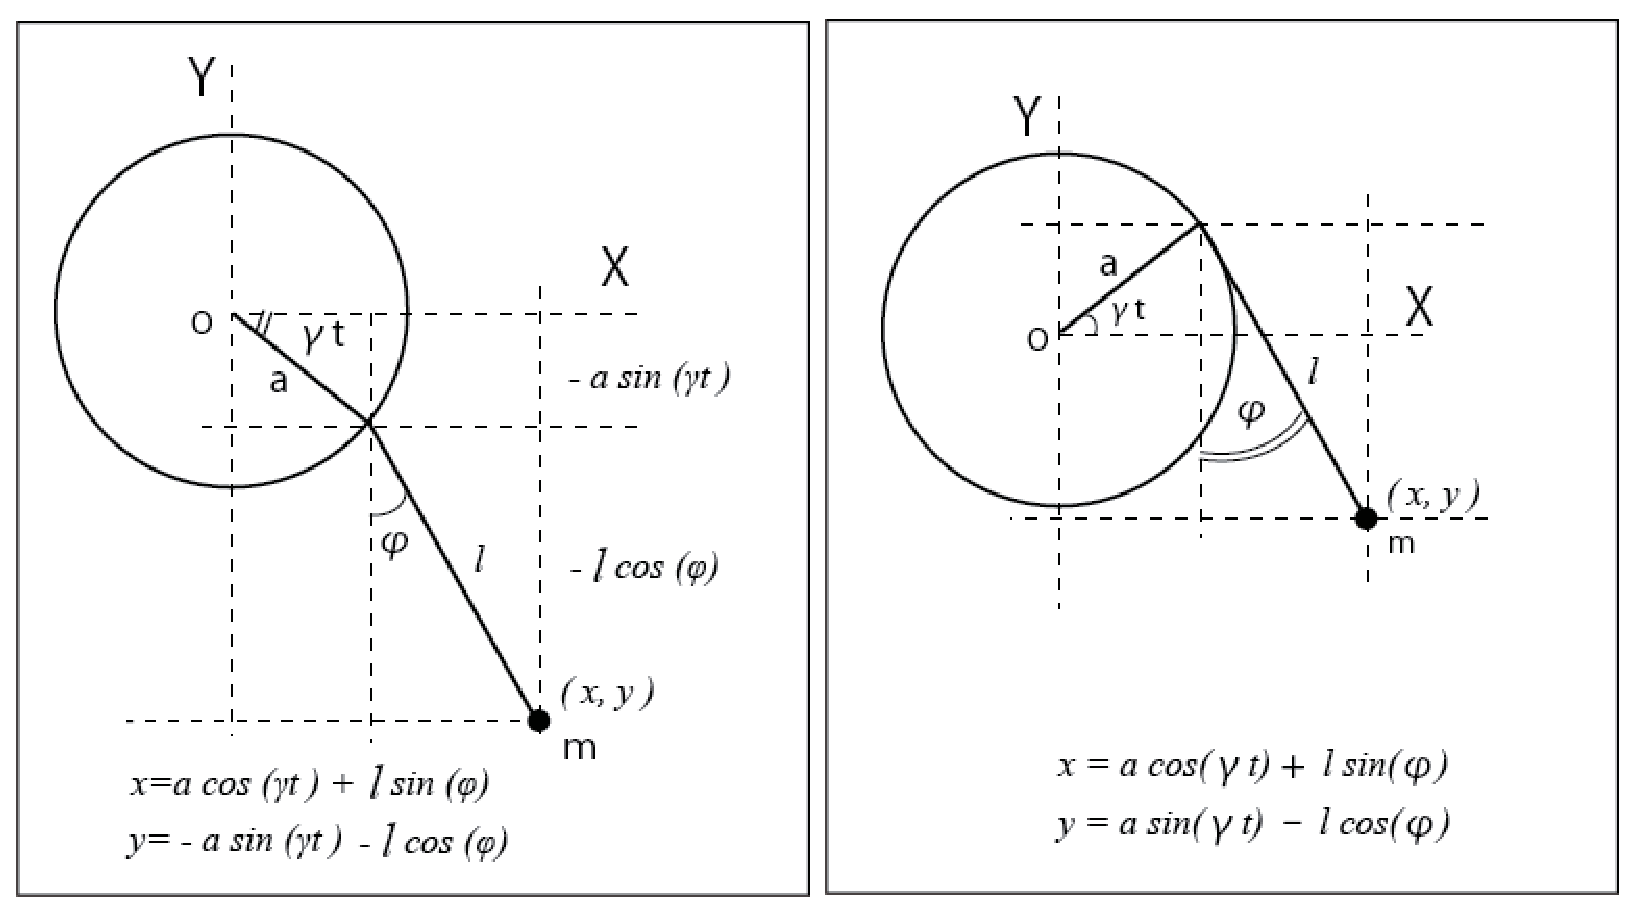
\includegraphics[keepaspectratio, scale=0.5]{eps/circular.eps}
          \caption{支点が円周上を周回する単振子}
        \end{minipage}
        %\begin{minipage}[b]{0.45\linewidth}
          %\centering
          %\includegraphics[keepaspectratio, scale=0.35]{p13-2.eps}
          %\caption{p13-2}
        %\end{minipage}
      \end{figure}
%\end{comment}

支点が鉛直平面内の円周上を一定の角速度$\gamma$で一様に動いている単振子. ($\gamma<0$でCW,$\gamma>0$でCCW,$\gamma$が$0$なら支点は動かない)

円周上の点に注目して($sin(-\gamma t)  = -sin(\gamma t)$だから)CWとCCWの違い

右の図は,CCW方向に回転する場合のモデル化になっている.質点$m$の位置$(x,y)$は,

\begin{align*}
   x&=a\cos\gamma t + l\sin\varphi\\
   y&=a\sin\gamma t - l\cos\varphi
\end{align*}

質点の速度,その自乗を作って,

\begin{align*}
   \dot{x}&=-a\gamma\sin\gamma t + l\dot{\varphi}\cos\varphi\\
   \dot{y}&=a\gamma\cos\gamma t + l\dot{\varphi}\sin\varphi\\
   \dot{x}^2&=a^2\gamma^2\sin^2\gamma t + l^2\dot{\varphi}^2\cos^2\varphi - 2al\gamma\dot{\varphi}\sin\gamma t\cos\varphi\\
   \dot{y}^2&=a^2\gamma^2\cos^2\gamma t + l^2\dot{\varphi}^2\sin^2\varphi + 2al\gamma\dot{\varphi}\sin\varphi\cos\gamma t
\end{align*}

運動エネルギー$T$とポテンシャル・エネルギー$U=mgy$は,

\begin{align*}
   T&=\displaystyle\frac{m}{2}\left(\dot{x}^2+\dot{y}^2\right)\\
   &=\frac{m}{2}\{a^2\gamma^2 + l^2\dot{\varphi}^2 + 2al\gamma\dot{\varphi}\left(\sin\varphi\cos\gamma t - \cos\varphi\sin\gamma t\right)\}\\
   &=\frac{m}{2}\{a^2\gamma^2 + l^2\dot{\varphi}^2 + 2al\gamma\dot{\varphi}\sin(\varphi-\gamma t)\}\\
   U&=mgy=mga\sin\gamma t - mgl\cos\varphi
\end{align*}

Lagrangian$L=T-U$は,

\begin{align*}
   L&=T-U\\
   &=\displaystyle\frac{m}{2}a^2\gamma^2 + \frac{m}{2}l^2\dot{\varphi}^2 + alm\gamma\dot{\varphi}\sin(\varphi-\gamma t) - mga\sin\gamma t + mgl\cos\varphi\\
   &=\frac{m}{2}l^2\dot{\varphi}^2 + alm\gamma\dot{\varphi}\sin(\varphi-\gamma t) + mgl\cos\varphi +\left(\frac{m}{2}a^2\gamma^2 - mga\sin\gamma t\right)
\end{align*}

右辺の最終項は, 次の関数$f(t)$の時間に関する完全導関数になっている.

\[f(t)=\displaystyle\frac{m}{2}a^2\gamma^2t + mga\frac{1}{\gamma}\cos\gamma t,\quad\frac{df(t)}{dt}=\frac{m}{2}a^2\gamma^2-mga\sin\gamma t\]

時間だけに依存する最終項を除けば,Lagrangianは最終的に次の様になる.(*座標と時間の任意の関数$f$の,時間に関する完全導関数$\dot{f}$をLagrangianの中に含んでいても,作用積分によってその変分は消えてしまう項になるので,取り除いても運動方程式としては変わらない.$\rightarrow$ランダウ「力学」p.5)

\[\therefore L=\displaystyle\frac{m}{2}l^2\dot{\varphi}^2 + alm\gamma\dot{\varphi}\sin(\varphi-\gamma t)+mgl\cos\varphi\]

次の計算をして,
\begin{align*}
   \displaystyle\frac{\partial L}{\partial\dot{\varphi}}&=ml^2\dot{\varphi} + alm\gamma\sin(\varphi-\gamma t)\\
   \displaystyle\frac{\partial L}{\partial\varphi}&=alm\gamma\dot{\varphi}\cos(\varphi-\gamma t)- mgl\sin\varphi
\end{align*}

もう少し準備して,

\[\displaystyle\frac{d}{dt}\frac{\partial L}{\partial\dot{\varphi}}=ml^2\ddot{\varphi}-alm\gamma^2\cos(\varphi-\gamma t)\]

Eular-Langange eq.

\[\displaystyle\frac{d}{dt}\frac{\partial L}{\partial\dot{\varphi}}-\frac{\partial L}{\partial\varphi}=0\]

は,

\[\therefore \ddot{\varphi}=\displaystyle\frac{a\gamma^2}{l}\cos(\varphi-\gamma t)+\frac{a\gamma}{l}\dot{\varphi}\cos(\varphi-\gamma t)-\frac{g}{l}\sin\varphi\]\\

一方, 左の図はCW方向に回転する場合のモデル化になっている.(実際, 右の図のモデルで$\gamma$を$-\gamma$で置き換えても同じ事になる.)質点$m$の位置$(x,y)$は,

\begin{align*}
   x&=a\cos\gamma t + l\sin\varphi\\
   y&=-a\sin\gamma t - l\cos\varphi
\end{align*}

質点の速度, その自乗と計算していくと,

\begin{align*}
   \dot{x}&=-a\gamma\sin\gamma t + l\dot{\varphi}\cos\varphi\\
   \dot{y}&=-a\gamma\cos\gamma t + l\dot{\varphi}\sin\varphi\\
   \dot{x}^2&=a^2\gamma^2\sin^2\gamma t + l^2\dot{\varphi}^2\cos^2\varphi - 2al\gamma\dot{\varphi}\sin\gamma t\cos\varphi\\
   \dot{y}^2&=a^2\gamma^2\cos^2\gamma t + l^2\dot{\varphi}^2\sin^2\varphi - 2al\gamma\dot{\varphi}\sin\varphi\cos\gamma t
\end{align*}

運動エネルギー$T$とポテンシャル・エネルギー$U$は,

\begin{align*}
   T&=\displaystyle\frac{m}{2}\left(\dot{x}^2+\dot{y}^2\right)\\
   &=\frac{m}{2}\{a^2\gamma^2 + l^2\dot{\varphi}^2 - 2al\gamma\dot{\varphi}\left(\sin\varphi\cos\gamma t + \cos\varphi\sin\gamma t\right)\}\\
   &=\frac{m}{2}\{a^2\gamma^2 + l^2\dot{\varphi}^2 - 2al\gamma\dot{\varphi}\sin(\varphi+\gamma t)\}\\
   U&=mgy= - mga\sin\gamma t - mgl\cos\varphi
\end{align*}

Lagrangian$L=T-U$は,

\begin{align*}
   L&=T-U\\&=\displaystyle\frac{m}{2}a^2\gamma^2 + \frac{m}{2}l^2\dot{\varphi}^2 - alm\gamma\dot{\varphi}\sin(\varphi+\gamma t) + mga\sin\gamma t + mgl\cos\varphi\\
   &=\frac{m}{2}l^2\dot{\varphi}^2 - alm\gamma\dot{\varphi}\sin(\varphi+\gamma t) + mgl\cos\varphi +\left(\frac{m}{2}a^2\gamma^2 + mga\sin\gamma t\right)
\end{align*}

右辺の最終項は, 次の関数$f(t)$の時間に関する完全導関数になっている.

\[f(t)=\displaystyle\frac{m}{2}a^2\gamma^2t - mga\frac{1}{\gamma}\cos\gamma t,\quad\frac{df(t)}{dt}=\frac{m}{2}a^2\gamma^2+mga\sin\gamma t\]

(*座標と時間の任意の関数$f$の,時間に関する完全導関数$\dot{f}$をLagrangianの中に含んでいても,作用積分によってその変分は消えてしまう項になるので,取り除いても運動方程式としては変わらない.$\rightarrow$ランダウ「力学」p.5)時間だけに依存する最終項を除けば,Lagrangianは最終的に次の様になる.

\[\therefore L=\displaystyle\frac{m}{2}l^2\dot{\varphi}^2 - alm\gamma\dot{\varphi}\sin(\varphi+\gamma t)+mgl\cos\varphi\]

次の計算をして,

\begin{align*}
   \displaystyle\frac{\partial L}{\partial\dot{\varphi}}&=ml^2\dot{\varphi} - alm\gamma\sin(\varphi+\gamma t)\\
   \displaystyle\frac{\partial L}{\partial\varphi}&=-alm\gamma\dot{\varphi}\cos(\varphi+\gamma t)- mgl\sin\varphi
\end{align*}

もう少し準備して,

\[\displaystyle\frac{d}{dt}\frac{\partial L}{\partial\dot{\varphi}}=ml^2\ddot{\varphi}-alm\gamma^2\cos(\varphi+\gamma t)\]

Eular-Langange eq.

\[\displaystyle\frac{d}{dt}\frac{\partial L}{\partial\dot{\varphi}}-\frac{\partial L}{\partial\varphi}=0\]

は,

\[\therefore \ddot{\varphi}=\displaystyle\frac{a\gamma^2}{l}\cos(\varphi+\gamma t)-\frac{a\gamma}{l}\dot{\varphi}\cos(\varphi+\gamma t)-\frac{g}{l}\sin\varphi\]

このCWの式は, CCWの場合のEular-Lgrange eq.の$\gamma$を$-\gamma$で置き換えて得られる式と同じ格好をしている.

\section{Pythonによる模擬実験}

連立の一階微分方程式に直して,関数ode定義する.右の図(CCWモデル)の場合のEular-Lagrange eq.からは,

\begin{align*}
   \displaystyle\frac{\mathrm{d}\varphi}{\mathrm{d}t}&=\dot{\varphi}\\\\
   \displaystyle\frac{\mathrm{d}\dot{\varphi}}{\mathrm{d}t}&=\displaystyle\frac{a\gamma^2}{l}\cos(\varphi-\gamma t) +\frac{a\gamma}{l}\dot{\varphi}\cos(\varphi-\gamma t)- \frac{g}{l}\sin\varphi
\end{align*}\\

円周上の点の位置$(x_0,y_0)$は、

\[x_0=a\cos\gamma t \quad,\quad y_0=a\sin\gamma t\]

であり、質点の位置$(x,y)$は、

\[x=x_0 + l\sin\varphi \qquad,\quad y=y_0 - l\cos\varphi\]

である.

左の図(CWモデル)の場合のEular-Lagrange eq.からは,

\begin{align*}
   \displaystyle\frac{\mathrm{d}\varphi}{\mathrm{d}t}&=\dot{\varphi}\\\\
   \displaystyle\frac{\mathrm{d}\dot{\varphi}}{\mathrm{d}t}&=\displaystyle\frac{a\gamma^2}{l}\cos(\varphi+\gamma t) -\frac{a\gamma}{l}\dot{\varphi}\cos(\varphi+\gamma t)- \frac{g}{l}\sin\varphi
\end{align*}

円周上の点の位置$(x_0,y_0)$は、

\[x_0=a\cos\gamma t \quad,\quad y_0=-a\sin\gamma t\]

であり、質点の位置$(x,y)$は、

\[x=x_0 + l\sin\varphi \qquad,\quad y=y_0 - l\cos\varphi\]

である.

模擬実験によって, CWとCCWの動きを確認することができる.わざわざ場合分けしてまでの記述をしているが, (当然の事ながら,) 一方の定式化だけにしておいて、定数GAMMAの符号を反転させても同じ現象になるよね.

\lstset{escapechar=@,style=custompy}
\lstinputlisting[caption=支点が円周上を周回する単振子,label=pythonProgram4]{py/circular.py}
